\documentclass[12pt, letterpaper]{article}
\usepackage[utf8]{inputenc}
\usepackage[margin=2cm]{geometry}
\usepackage{amsmath}
\usepackage{amssymb}
\usepackage{graphicx}
\usepackage{cancel}
\usepackage{fancyhdr}

\graphicspath{ {./bilder/} }
\title{Portfolio assignment 2}
\author{Candidate25}
\date{}

\rfoot{\thepage}
\newcommand{\bs}{\boldsymbol}
\newcommand{\mbf}{\mathbf}

\maketitle
\begin{document}
  \section*{Problem 1}
    \subsection*{(1a)}
      \begin{figure}[h]
        \caption{Decision boudary of a logistic descrimination classifier}
        \centering
        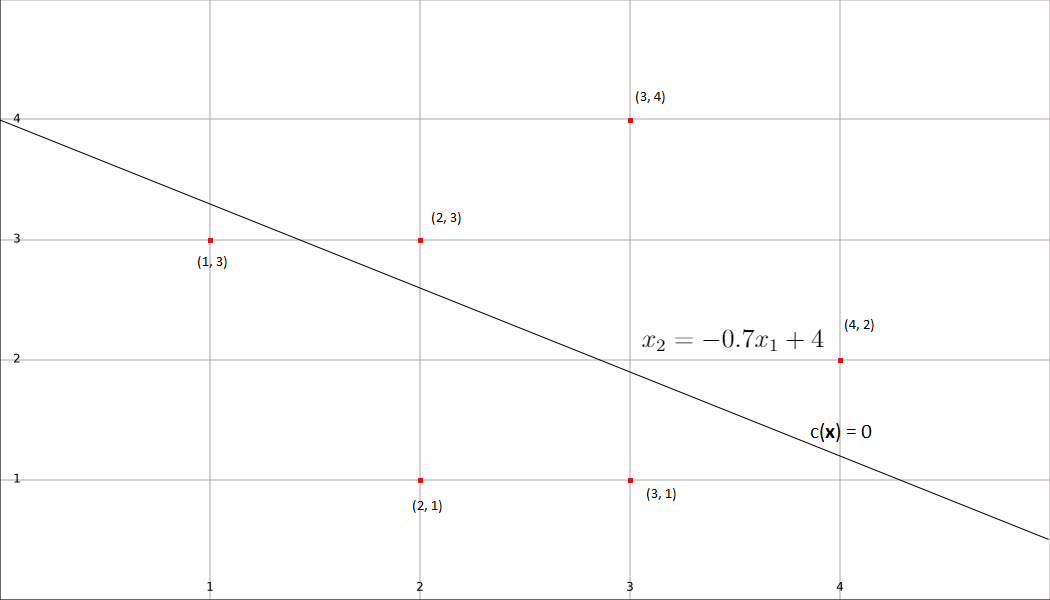
\includegraphics[width=\textwidth,keepaspectratio=true,height=\textheight-\the\textundbildtextheight]{decisionboundary_1a}
      \end{figure}\\
      In the plot above we see the points from the training set: $\{(\mbf{x}^i, y^i)\}_{i=1}^6$ as red points. $\mbf{x}^i$ is the trainig data, and $y^i$ is the ground truth. The line going somewhat diagonally across the plot is the decision boundary. This is used to classify the points above the line as $y^i = 0$, and points underneath the decision boundary as $y^i = 1$. This decision boundary is given by the equation:
      \begin{align} \label{eq1}
        C(\mbf{x}) = \bs{w}^T \cdot \mbf{x} + w_0
      \end{align}
      Which put simply, assigns a class to an vector $\mbf{x}^i$. If the vector after being put into\\ $C(\mbf{x}) > 0 \implies \mbf{x} \rightarrow C^1$ or the opposite case where $C(\mbf{x}) < 0 \implies \mbf{x} \rightarrow C^2$. Which means at $C(\mbf{x}) = 0$ we are on the decision boundary. From this we can derive the equation of the decision boundary, $x_2 = -\frac{w_1}{w_2}\cdot x_1 - \frac{w_0}{w_2}$. In my guess for the decision boundary i used $w_1 = -0.7, w_2 = 1$ and $ w_0 = 4$ to give the decision boundary of $x_2 = -0.7 \cdot x_1 + 4$. Here we see that the weights, $\bs{w}$ of the classifier determines the slope of the decision boundary, whereas the bias, $w_0$ determines the intercept with the second axis, $x_2$.\\
      \newline
      To figure out the distance between the origin, $\bs{O}$, and the decision boundary we can calulate this with the formula,
      \begin{align*}
        d = \frac{w_0}{\|\bs{w}\|} = \frac{4}{\sqrt{(-0.7)^2 + 1^2}} \approx \underline{\underline{3,277}}
      \end{align*}\\
      Now i shall demonstrate how this decision boundary could give us a decision rule, based on the estimated weights and biases. Consider a test point,
      \begin{align*}
        \mbf{x}^t =
        \begin{bmatrix}
          x_1^t \\
          x_2^t \\
        \end{bmatrix}
      \end{align*}
      this point will from what I stated earlier follow the  decision rule,
      \[
        \begin{cases}
          C(\mbf{x^t}) > 0, & y^t = 0\\
          C(\mbf{x^t}) \leq 0, & y^t = 1\\
        \end{cases}
      \]
      Here i have also made the assumption that if  $C(\mbf{x^t}) = 0$ then $\mbf{x^t}$ is assigned to $y^t = 1$, althoug in reality this is quite rare.

    \subsection*{(1b)}
      % \begin{figure}[h]
      %   \caption{Confusion matrix and accuracy of test on trained model.}
      %   \centering
      %   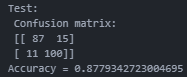
\includegraphics[width=5cm]{confmat1b}
      % \end{figure}
      After having trained my logistic discrimination model on the \textit{seals\_train.csv} file, and the used the trained weights to classify the test data. I produce with the \textit{seals\_test.csv} file the confusion matrix:\\
      \[
        \text{confusion matrix} =
        \begin{bmatrix}
          87 & 15  & \\
          11 & 100 & \\
        \end{bmatrix}
        \text{, and accuracy} \approx \underline{0.878}
      \]
      Which means the model classified 87 class 0's correctly, 11 class 1's as class 0's, 15 class 0's as class 1's and 100 class 1's correctly.
    \newpage
    \subsection*{(1c)}
    \begin{figure}[h]
      \caption{The Reciever Operating Characteristic}
      \centering
      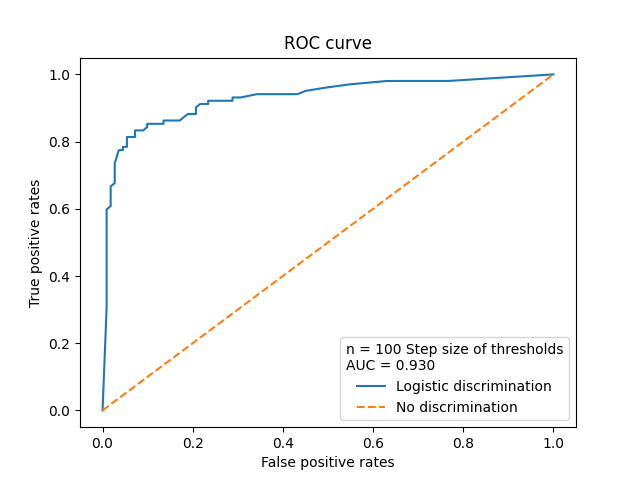
\includegraphics[width=14cm]{ROC}
    \end{figure}\\
    The ROC curve represents\\

    For the Area Under the Curve score i got AUC $ \approx \underline{0.930}$ by using \textit{sklearn.metrics} built-in function for calculating the AUC score.
\end{document}
